\subsection{第 3 课}

\subsubsection{脑图}

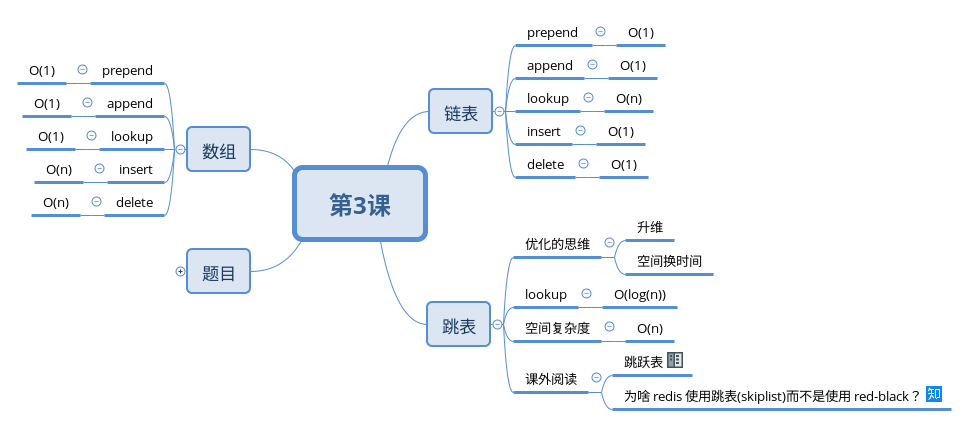
\includegraphics[width=170mm,height=80mm]{images/第3课.png}

\subsubsection{题目}

\paragraph{Array 实战题目}

\begin{itemize}
  \item \hyperref[leetcode:11]{11. 盛最多水的容器}
  \item \hyperref[leetcode:283]{283. 移动零}
  \item \hyperref[leetcode:70]{70. 爬楼梯}
  \item \hyperref[leetcode:15]{15. 三数之和}
\end{itemize}

\paragraph{Link List 实战题目}

\begin{itemize}
  \item \hyperref[leetcode:206]{206. 反转链表}
  \item \hyperref[leetcode:24]{24. 两两交换链表中的节点}
  \item \hyperref[leetcode:141]{141. 环形链表}
  \item \hyperref[leetcode:142]{142. 环形链表 II}
  \item \hyperref[leetcode:25]{25. K 个一组翻转链表}
\end{itemize}

\paragraph{课后作业}

\begin{itemize}
  \item \hyperref[leetcode:26]{26. 删除排序数组中的重复项}
  \item \hyperref[leetcode:189]{189. 旋转数组}
  \item \hyperref[leetcode:21]{21. 合并两个有序链表}
  \item \hyperref[leetcode:88]{88. 合并两个有序数组}
  \item \hyperref[leetcode:1]{1. 两数之和}
  \item \hyperref[leetcode:283]{283. 移动零}
  \item \hyperref[leetcode:66]{66. 加一}
\end{itemize}
